% Template for PLoS
% Version 1.0 January 2009
%
% To compile to pdf, run:
% latex plos.template
% bibtex plos.template
% latex plos.template
% latex plos.template
% dvipdf plos.template

\documentclass[10pt]{article}

% amsmath package, useful for mathematical formulas
\usepackage{amsmath}
% amssymb package, useful for mathematical symbols
\usepackage{amssymb}

% graphicx package, useful for including eps and pdf graphics
% include graphics with the command \includegraphics
\usepackage{graphicx}

% cite package, to clean up citations in the main text. Do not remove.
\usepackage{cite}

\usepackage{color}

% Use doublespacing - comment out for single spacing
%\usepackage{setspace}
%\doublespacing


% Text layout
\topmargin 0.0cm
\oddsidemargin 0.5cm
\evensidemargin 0.5cm
\textwidth 16cm
\textheight 21cm

% Bold the 'Figure #' in the caption and separate it with a period
% Captions will be left justified
\usepackage[labelfont=bf,labelsep=period,justification=raggedright]{caption}

% Use the PLoS provided bibtex style
\bibliographystyle{plos2009}

% Remove brackets from numbering in List of References
\makeatletter
\renewcommand{\@biblabel}[1]{\quad#1.}
\makeatother


% Leave date blank
\date{}

\pagestyle{myheadings}
%% ** EDIT HERE **


%% ** EDIT HERE **
%% PLEASE INCLUDE ALL MACROS BELOW

%% END MACROS SECTION

\begin{document}

% Title must be 150 characters or less
\begin{flushleft}
{\Large
\textbf{A bioinformatics pipeline for the analysis and interpretation of ultradeep sequence data}
}
% Insert Author names, affiliations and corresponding author email.
\\
N Lance Hepler$^{1,\ast}$,
Martin D Smith$^{1}$
Wayne Delport$^{2}$,
Jason A Young$^{3}$,
Art FY Poon$^{4}$,
Sergei L Kosakovsky Pond$^{3}$
\\
\bf{1} Interdisciplinary Bioinformatics and Systems Biology Program, University of California San Diego, La Jolla, California, USA
\\
\bf{2} Prognosys Biosciences, La Jolla, California, USA
\\
\bf{3} Department of Medicine, University of California San Diego, La Jolla, California, USA
\\
\bf{4} BC Centre for Excellence in HIV/AIDS, Vancouver, British Columbia, Canada
\\
$\ast$ E-mail: Corresponding nhepler@ucsd.edu
\end{flushleft}

% Please keep the abstract between 250 and 300 words
\section*{Abstract}
\textbf{Background:} Massively parallel sequencing technologies are increasingly adopted for the study of rapidly evolving and diverse pathogens, such as HIV-1.
Custom bioinformatics tools are needed to address domain-specific challenges of viral sequence analysis
and differentiate sequencing artifacts from biologically meaningful mutations.
Large quantities of data require parallelized and efficient algorithms for rapid analysis.

\textbf{Results:} We have developed simple probabilistic methods to model ultradeep sequencing errors
and implemented a web-based (http://www.datamonkey.org)
and standalone analysis pipeline to facilitate common analyses of HIV-1 sequence data generated using the Roche 454 platform.
Such analyses include robust read mapping and filtering,
instrument error filtering,
identification of drug-resistance associated and accessory mutations,
diversity estimation,
determination of whether a host is multiply infected,
and the computation of simple measures of selective pressures on individual sites. 

\textbf{Conclusions:} Our pipeline is designed to provide end-users with the tools to rapidly analyze sequences derived
from the Roche 454 sequencing platform and is geared specifically for the analysis of HIV-1 and other rapidly evolving RNA viruses.


% Please keep the Author Summary between 150 and 200 words
% Use first person. PLoS ONE authors please skip this step.
% Author Summary not valid for PLoS ONE submissions.
\section*{Author Summary}

\section*{Introduction}
Recent advances in DNA sequencing technology have facilitated the generation of massive amounts of data,
the utility of which is entirely dependent on the analysis tools available to researchers.
Ultradeep sequencing projects utilizing the Roche 454 Titanium FLX platform (the 454 platform)
routinely generate tens or hunderds of thousands of reads from multiple genes and samples.
In the context of HIV-1,
these data have proven useful in studies of evolution of drug resistance \cite{Wang2007,Hoffmann2007},
response to host immune pressure \cite{Bimber2009,Hughes2010,Poon2010,Love2010},
co-receptor usage \cite{Archer2009,Tsibris2009} and the dynamics of acute infection \cite{Fischer2010}.
A major advantage of ultradeep sequencing platforms is their power to detect low-frequency, or minority, genetic variants.
Population-based sequencing of plasma samples has been shown to be inefficient at identifying variants with prevalence less than 10\% \cite{Palmer2005},
whereas minority variants at frequencies below 1\% have been recovered using ultradeep sequencing methods \cite{Zagordi2010}.
Given that circulating or archived minority variants can cause antiretroviral therapy failure \cite{Palmer2006,Lecossier2005,Kapoor2004},
high-resolution sequence characterization of viral populations is desirable,
particularly within the context of drug resistance and treatment.
However, in doing so care must be taken in distinguishing true biological minority variants from artifactual variants arising due to PCR and sequencing errors.
PCR misincorporation can introduce mutations at a rate of $10^{-5}$ to $10^{-4}$ \cite{Kobayashi1999},
whereas base-calling and other 454 platform-specific errors are typically larger
in regions containing repeats of three of more identical nucleotides (homopolymers)\cite{Wang2007}.
One approach to quantify ultradeep sequencing error has been to sequence clonal samples \cite{Wang2007},
which suggested 0.0007 and 0.0044 mismatch errors per nucleotide sequenced in non-homopolymeric and homopolymeric regions, respectively.
Since error rates are likely to be sample- and gene-specific,
and since it is infeasible to obtain clonal control sequencing runs for all samples in a study,
it is necessary to devise metrics for the detection of ultradeep sequence errors in a sample specific manner.
To that end, we have developed simple methods to model ultradeep sequence errors
and assembled an analysis pipeline to facilitate common analyses of HIV-1 sequence data generated using the 454 platform.


% Results and Discussion can be combined.
\section*{Results}

To illustrate the pipeline we present some results derived
from a multiplexed 454 sequence data covering regions in \textit{gag}, \textit{rt} and \textit{env}
from a single plasma sample extraction.
This sample was one of those recently analyzed for evidence of dual HIV infection \cite{Pacold2010}.

\subsection*{Alignment filtering and sequence diversity}
Quality filtering with a PHRED score of 20 and minimum read length of 100 reduced the total number of reads from 19996 to 19377.
However, since we split reads with internal regions of low quality,
a total of 23824 high-scoring fragments were retained for subsequent analyses.
Of these fragments, the majority mapped to the \textit{env} reference sequence,
followed by \textit{gag} and \textit{rt} (Table~\ref{summarystats}).
In addition to these summary statistics,
we produce plots of coverage and majority variants proportions along each gene region (Figure~\ref{coverageFig})
to facilitate the rapid identification of regions of insufficient data quantity.
Furthermore, the majority variant plots provide a means to identify regions of high diversity
which may want to be targeted in subsequent ultradeep sequencing experiments.
All plots are indexed according to the reference sequence (either HIV-1 or a custom upload),
and are available for download from the server.
Sliding windows of maximum sequence diversity, and neighbor-joining trees,
further allow the user to identify regions of increased diversity,
or in the case of HIV-1, identify poly-clonal infection (as in \cite{Pacold2010}).
Since ultradeep sequence reads are typically short,
and thus contain very little phylogenetic signal,
we only estimate bootstrap support for neighbor-joining trees in the sliding window of maximum diversity.
In most cases, however, there is little bootstrap support for any particular branching order in the tree.

\subsection*{Sequence alignment}
XXX TODO

\subsection*{Estimation of 454 sequence error and mutation rate classes}
Our binomial mixture model identified strong evidence for multiple mutation rate classes
in all three genes with substantial AIC improvements in all cases (Table~\ref{rateclasses}).
\textbf{Assuming the lowest estimated mutation rate is the background mutation rate,
we are able to identify sites that mutate at higher rates.}
In some cases (as in site 234) the identification of true mutations is trivial,
particularly when several variants occur at intermediate to high frequencies (Figure~\ref{sitesFig}).
However, we frequently need to distinguish minority variants from sequencing error,
particularly when the former occur at frequencies less than 1\%.
For instance, sites 250 and 251 (Figure~\ref{sitesFig}) are assigned to the background mutation rate class (in this case with rate = 0.002),
whereas other sites (such as 262) with similar levels of diversity are assigned to a higher rate class.
Given the coverage at a site, we can estimate the probability of observing $m$ mutations assuming the background mutation rate (0.002 for \emph{env})
using a binomial model (Figure~\ref{sitesFig}).
These results allow for the determination of whether allelic variants at a site
are likely to be the result of sequencing error.
This delineation is particularly important in the context of HIV minority drug resistance
and thus we utilize the same statistical tools to identify both sites,
and variants at sites which can be separated from sequencing error.
Results for all sites are presented as HTML pages
and are also available as downloadable comma-separated value files for further processing.

\section*{Discussion}
Our pipeline is designed to provide end-users with the tools to rapidly analyze sequences derived
from the 454 ultradeep sequencing platform and is geared specifically for the analysis of rapidly evolving populations, such as RNA viruses.
We provide tools to rapidly filter reads based on reference sequences,
to identify sequence variants within sliding windows,
to identify allelic variants at sites,
and to distinguish biologically meaningful variants from sequencing error artifacts.
Estimates of site-specific purifying and diversifying selection are calculated,
as are several statistics which facilitate the interpretation of sequence variation among ultradeep sequence reads.
Finally, for HIV-1 sequence data we provide tools for the identification of polymorphisms at known drug-resistant sites.
All these analyses tools are provided through an intuitive user-friendly interface at http://www.datamonkey.org
and complement the array of other evolutionary biology tools available at our webserver.
A standalone version of the pipeline is also provided, along with supporting documentation online.

% You may title this section "Methods" or "Models".
% "Models" is not a valid title for PLoS ONE authors. However, PLoS ONE
% authors may use "Analysis"
\section*{Methods}
The HIV-1 analysis pipeline has been implemented as a HyPhy \cite{KosakovskyPond2005} Batch Language module,
and on the Datamonkey webserver (http://www.datamonkey.org) \cite{KosakovskyPond2005a,Delport2010}.
The pipeline comprises several phases,
each of which interacts with a SQLite database (http://www.sqlite.org) backend for results storage and processing.
Phases which can benefit from execution in parallel (e.g. read mapping) have been implemented to make use of distributed computing environments which use MPI.

\subsection*{Quality filtering of reads}
The analysis pipeline takes as input two files generated from a 454 sequencing experiment,
the read file (.fna) in FASTA format (required), and the quality file (.qual) with site specific quality scores (q or PHRED)
for each of the reads in the read file (optional).
By default, reads that are least 100 nucleotides long and have consecutive quality scores of 20 or greater are retained for subsequent analysis.
These, and most other analysis parameters can be modified by the user.
A quality score of 20 is interpreted as equivalent to one error in 100 bases (XXX) \cite{}.
Errors in 454 pyrosequencing are frequently the result of incorrect determination of homopolymer lengths \cite{Wang2007}.
We make a special allowance for such regions to be excised by breaking a longer read with a poor quality score section in the middle into multiple fragments,
each of which must meet the minimum length and quality score criteria.

\subsection*{Sequence alignment}
We use an iterative gene-specific alignment and filtering procedure.
Firstly, we define a reference sequence, or set of reference sequences,
which is used to filter ``mappable'' reads from the set of reads identified by the quality filtering step described above.
A 454 sequencing run can include multiple amplicons of different gene regions without the need for multiplexing tags.
Therefore, we provide a list of HIV-1 reference genes (HXB2, GenBank accession number K03455) which are initially used as a mapping reference.
Alternatively, a custom reference sequence file can be uploaded.
XXX REWRITE THIS ENTIRE SECTION {
Every read is translated into six protein sequences: one in each of the six (three forward and three reverse complement) reading frames.
Encountered stop codons are mapped to the letter 'X' which is functionally equivalent to a missing base for the subsequence alignment phase.
Next, each translation is locally aligned \cite{Needleman1970} to the currently considered HXB2 gene,
using an HIV-specific scoring matrix \cite{Nickle2007}.
The reading frame with the highest alignment score is retained for subsequent steps.
The reads are further filtered to select High Protein-Alignment Scoring (HPAS) reads,
defined as reads whose \textit{per-residue} alignment scores exceed the expected alignment score of a random sequence
with sample-specific base composition by at least X-fold.
$X=5$ yielded good filtering properties on synthetic data;
this translates, roughly, into a $\log_{2} 5$ informative bits per position (conceptually similar to BLAST bit scores).
The consensus codon sequence of mapped HPAS reads is constructed and used as a sample-specific reference sequence from this point onwards.
The remaining sequences, i.e. those not selected for the HPAS, are subsequently nucleotide aligned to the HPAS reference,
and included if their alignment scores exceeds the median score of the distribution of HPAS reads.
This nucleotide alignment step permits the correction of out-of-frame indels or homopolymer length errors specific to the 454 platform.
}

\subsection*{Estimation of divergence}
In order to identify distinct viral populations,
e.g. in the context of dual infection \cite{Pacold2010},
we estimate maximum sequence divergence in sliding windows with a default width and stride of 125 and 25 nucleotides, respectively.
For each sliding window with minimum site coverage greater than a pre-defined value (default = 500),
we estimate sequence divergence using the general time reversible model of nucleotide evolution \cite{Tavare86},
along the phylogeny inferred using the Neighbor Joining method\cite{Saitou1987}.
Nucleotide diversity is determined as the maximum path length in the tree with branch lengths estimated by maximum likelihood.
For this analysis, we require that a sequence variant occur at least $N$ times ($10$ by default),
or comprise at least $P\%$ of the sample (1\% by default), whichever is greater, to be considered a non-artifactual variant.
We determine statistical support for internal nodes, and maximum sequence diversity, using bootstrap over alignment sites (100 replicates).

\subsection*{Estimation of 454 sequence error and mutation rate classes}
In order to estimate a sample-specific 454 sequence error rate,
and thus a threshold for the identification of biologically meaningful minority polymorphisms at a site,
we fit a binomial mixture model to site-specific mutation counts.
A binomial distribution (albeit with an \textit{a priori} error rate)
has been suggested as a good PCR noise filtering model in the context of conservation genetics \cite{Cummings2010}.
At site $i$ from a 454 sample with coverage, $c_{i}$, the probability of observing exactly $m_{i}$ mutations
(identified as non-consensus amino acid residues at a site) assuming the binomial model is given by
\begin{equation}
L(D_{i}|r_{1}) = \binom{c_{i}}{m_{i}}r_{1}^{m_{i}}(1-r_{1})^{c_{i}-m_{i}},
\end{equation}
where the parameter, $r_{1}$---interpreted as the mutation rate at a site---is estimated by maximum likelihood as the proportion of observed counts.
Assuming each site in an alignment is independent,
the mean mutation rate can similarly be estimated for all sites as the product of site likelihoods using maximum likelihood, i.e.
\begin{equation}
L(D|r_{1}) = \prod_{i=1}^{s}  L(D_{i}|r_{1}),
\end{equation}
where $s$ is the number of sites.
We next consider a mixture model of $K$ binomial distributions (each with its own rate $r_{j}$).
The likelihood of mutation data under this model is given by
\begin{equation}
L(D) = \prod_{i=1}^{s}  \sum_{j=1}^{K} p_{j} L(D|r_{j}),
\end{equation}
where $p_{j}$, $\sum_{j} p_{j} = 1$, are the mixing proportions.
The goodness-of-fit for each model is evaluating using Akaike Information Criterion (AIC).
Beginning with $K=1$, we increment the number of rate classes by one,
until the model with $K+1$ rates is no longer preferred to the model with $K$ rates by AIC.
The mutation rates (and respective proportions) for each of the rate classes are presented,
as are the improvements in model fit with the addition of rate classes.

Next, we \textit{assume} that the class with the lowest mutation rate, $r_{e}$, represents sites subject to sequencing or instrument errors.
This mutation rate can be used as a sample specific threshold for the identification of minority variants.
More generally, we use an empirical Bayes procedure to obtain the posterior probability that site $i$ is assigned to rate class $j$ via
\begin{equation}
P(r_{j}|D_{i}) = {L(D_{i}|r_{j}) P(r_{j}) \over { \sum_{a=1}^{k} L(D_{i}|r_{a}) } P(r_{a})},
\end{equation}
where $P(r_{j}) = p_{j}$ is the prior probability that site $i$ belongs to rate class $j$.
This approach is an improvement over \textit{a priori} percentage or count-based thresholds,
since it is dependent on both the depth (coverage) in an alignment,
and on sample specific mutation patterns which are likely to vary between alignments (XXX) \cite{}.
In addition to estimating the number of mutation rate classes supported by the data,
we estimate the observed mutation rates at each of the sites in the alignment.
Given a site with coverage, $c$, we estimate the effective mutation rate
as the number of non-consensus amino acids, $n$, normalized by the coverage (i.e. $n / c$).

At every site, we record the amino acid spectrum, $A = (c_{A}, \ldots, c_{Y}$),
where the index iterates through the twenty amino acids and $c_{X}$ denotes the count of amino acid, $X$, at the site.
For visualization and data exploration purposes, we calculate the Shannon entropy at site $s$, $H(s)$,
\[H (s) = -\sum_{X, f_{s}(X)\ne 0} f_s(X) \log {f_{s}(X)},\] where $f_s(X)$ is the proportion of reads with residue $X$ at site $s$,
and the sum is taken over observed residues only.

\subsection*{Sitewise estimation of diversifying and purifying selection}
Typically estimates of diversifying and purifying selection are conditional on a known phylogeny (see \cite{Delport2009,Anisimova2009} for reviews).
However, since ultradeep sequences from single 454 samples typically contain relatively short reads (200--300 bp) with low diversity ($<0.05$),
the phylogenies estimated from the data have little statistical support.
Therefore, we estimate selection at a site by considering the ratio of expected non-synonymous and synonymous mutations assuming neutral evolution,
given the genetic code and observed codon frequencies, following the procedure outlined in detail in \cite{KosakovskyPond2005b}.
We also evaluate the ratio of the \textit{observed} non-synonymous to synonymous substitutions at a site, by considering, for every read,
the mean numbers of synonymous ($s$) and non-synonymous substitutions ($n$)
along the shortest evolutionary path connecting it to every other read (i.e. $c-1$ possibilities, for $c$ reads covering the site).
This is equivalent to assuming a complete lack of phylogenetic information,
i.e. any sequence is equally likely to be ancestral to any other sequence.
Significance is assessed using the binomial distribution, \[ \binom{c}{s}p_{s}^{s}(1-p_{s})^{c-s}, \]
as the probability of observing $s$ or fewer synonymous substitutions out of $c=n+s$ total substitutions
given an expected proportion of synonymous substitution, $p_{s}$, under neutrality.

\subsection*{Identification of Drug Resistant Variants}
We screen for the occurrence of mutations in reverse transcriptase (\textit{rt}), integrase (\textit{int}) and protease (\textit{pr}),
that are known to confer resistance to antiretroviral agents (`drug resistance associated mutation' or DRAM sites).
A current comprehensive list of such mutations is maintained at the Stanford HIV drug resistance database (http://hivdb.stanford.edu) \cite{Shafer2006}.
For each DRAM site we rank its mutation rate with respect to all other sites (on a 0--100\% scale),
and calculate the median mutation rank of all non-DRAM sites.
Given this median rank, we determine whether it is significantly elevated compared to that of non-drug resistant sites,
using equivalently-sized random subsamples ($n=1000$) from sites not known to be directly associated with drug resistance.
Such an elevation could indicate that selective forces are preferentially acting upon DRAM sites on average.
We bin drug resistant sites into the estimated mutation rate classes to distinguish biologically and clinically relevant minority variants
from those arising due to instrument error.
Finally, we screen for known compensatory (accessory) mutations
with the purpose of identifying whether these co-occur more frequently with known drug resistant variants than expected by chance.
Such linkage between drug resistant and accessory mutations in the sample provides corroborating evidence that detected DRAMs are not artifactual.

% Do NOT remove this, even if you are not including acknowledgments
\section*{Acknowledgments}


%\section*{References}
% The bibtex filename
\bibliography{plos}

\section*{Figure Legends}
\begin{figure}[!ht]
\begin{center}
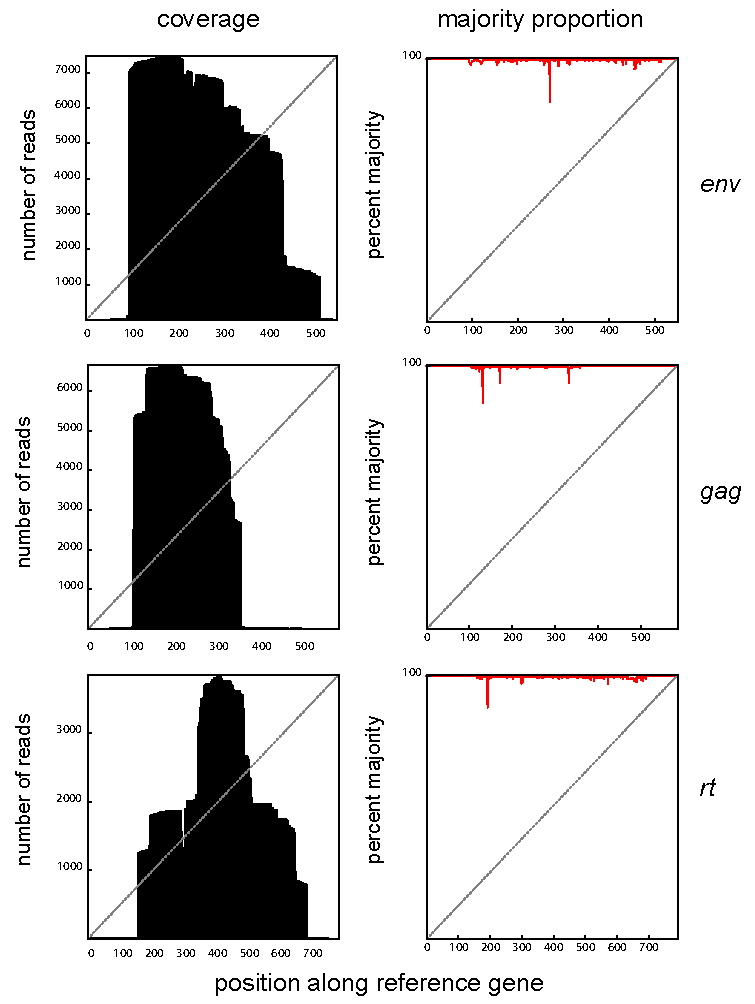
\includegraphics[width=4in]{figures/coverage.pdf}
\end{center}
\caption{
{\bf Site-specific coverage and majority variants obtained in a single 454 run containing \textit{env}, \textit{gag}, and \textit{rt} amplicons.}
}
\label{coverageFig}
\end{figure}

\begin{figure}[!ht]
\begin{center}
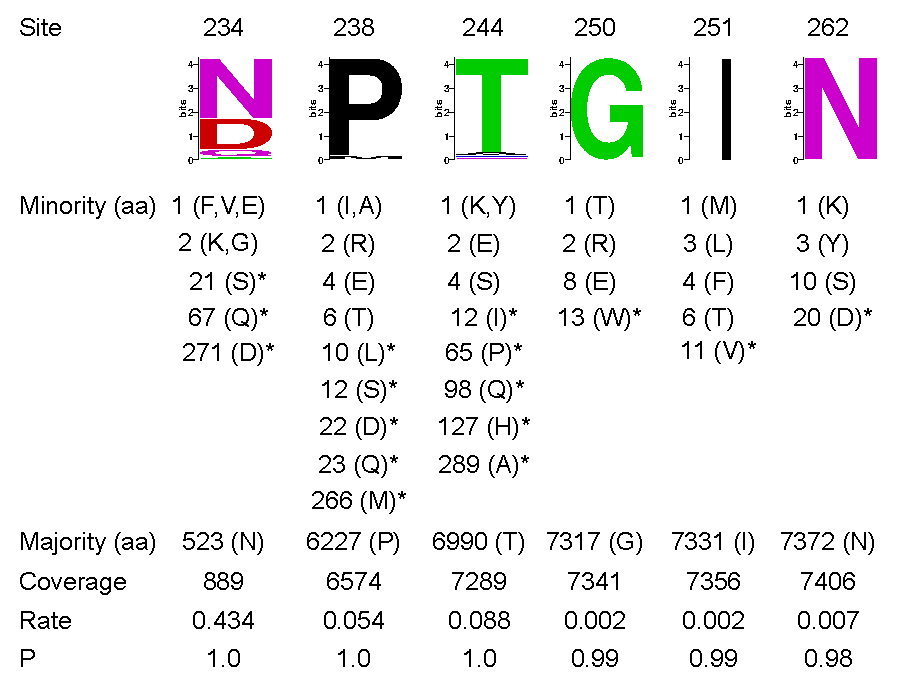
\includegraphics[width=4in]{figures/siterates.pdf}
\end{center}
\caption{
{\bf Assignment of \textit{env} sites to rate classes based on a binomial mixture model.}
Examples of sites with intermediate and low-frequency variants
are shown to demonstrate the ability of the model to distinguish mutations at a site
from a background (or 454 error) mutation rate.
Shown are the amino acid profiles, the coverage,
the mutation rate of the class to which the site is assigned,
and the posterior probability, $P$, that the site belongs to the assigned rate class.
* Indicates significance ($P \leq 0.05$) for a test of whether the $n$ observed mutations are expected to occur
given the estimated background mutation rate (0.002) and the coverage at a site.
}
\label{Figure_label}
\end{figure}

\section*{Tables}
\begin{table}[!ht]
\caption{
\bf{Summary read statistics from a 454 sample containing \textit{env}, \textit{gag}, and \textit{rt} sequences (sd = standard deviation)}}
\begin{tabular}{lccccc}
gene & reads & mean read length & sd read length & mean coverage at a site & sd coverage\\
\hline
\textit{env} & 8620 & 266.37 & 92.65 & 4182.46 & 2992.71 \\
\textit{gag} & 6728 & 214.48 & 40.26 & 2466.65 & 2921.27 \\
\textit{rt}  & 6683 & 179.64 & 66.70 & 1521.62 & 1304.18 \\
\hline
\end{tabular}
\begin{flushleft}
\end{flushleft}
\label{table:summarystats}
\end{table}

\begin{table}[!ht]
\caption{
\bf{Mutation rate classes estimated using the binomial mixture model}}
\begin{tabular}{lcccc}
gene & number of rate classes & mutation rates range & proportion background & $AIC_{i}$ \\
\hline
\textit{env} & 8 & 0.002--0.434 & 0.55 & 28032.36 \\
\textit{gag} & 4 & 0.002--0.175 & 0.84 & 13756.25 \\
\textit{rt}  & 5 & 0.002--0.126 & 0.46 &  5938.45 \\
\end{tabular}
\begin{flushleft}
$AIC_{i}$ is the improvement in fit over a single-rate model;
proportion background is the proportion of sites
which are assigned to the background,
or the smallest estimated mutation rate.
\end{flushleft}
\label{table:rateclasses}
\end{table}

\end{document}

